\documentclass[11pt]{article}
\usepackage{geometry}                % See geometry.pdf to learn the layout options. There are lots.
\geometry{letterpaper}                   % ... or a4paper or a5paper or ... 
%\geometry{landscape}                % Activate for for rotated page geometry
%\usepackage[parfill]{parskip}    % Activate to begin paragraphs with an empty line rather than an indent
\usepackage{graphicx}
\usepackage{amssymb}
\usepackage{epstopdf}
\usepackage{cite}

\DeclareGraphicsRule{.tif}{png}{.png}{`convert #1 `dirname #1`/`basename #1 .tif`.png}

\title{Gadgetron - A General Purpose Image Reconstruction and Processing Framework}
\author{Michael S. Hansen - michael.hansen@nih.gov \\ Thomas S. S{\o}rensen - sangild@cs.au.dk}
\date{}

\begin{document}
\maketitle
\tableofcontents

\section{Introduction}
The Gadgetron framework is a streaming data processing framework developed for medical image reconstruction. It has been developed as a tool to prototype, test, and deploy novel image reconstruction algorithms. The framework also contains several toolboxes with data structures and algorithm, which can be used within the streaming framework or in standalone applications. This document serves as a very brief introduction to the framework and gives a few examples of using the framework. In addition to this document, source code documentation is provided with the framework.

Initially this framework was developed to support the work of the authors in the field of advanced MRI reconstruction, and specifically to support work on fast image reconstruction not only on traditional CPU architecture but also using commodity graphics hardware (GPUs). Over the years we have developed and published several journal papers in this field. Some examples include fast regridding on the GPU  \cite{sorensen_accelerating_2008} and parallel Cartesian parallel imaging \cite{hansen_cartesian_2008}. 

%\subsection{History}
%\subsection{Target Applications}
%\subsection{Example Usage}

\section{Getting Started}
\subsection{Prerequisites}
The Gadgetron framework is built on the ADAPTIVE Computing Environment (ACE)\footnote{ACE can be downloaded from XXX.com and a good tutorial of ACE can be found at YYY.com}. It is not necessary to be familiar with ACE, but it certainly is an advantage since all objects and datatypes are inherited from ACE. 

\subsection{Obtaining Gadgetron}

\section{Architecture}

\subsection{Overview}
The \emph{Gadgetron} is a streaming framework for image processing. The data processing stream is comprised of more or more \emph{Gadgets} that each implement part of the data processing pipeline. Data enters tha Gadgetron through a tcp/ip socket interface and is passed down the chain of Gadgets. An overview of the system is shown in figure \ref{fig:architecture}. A number of \emph{Readers} are responsible for reading the input on the socket. In practice different Readers are associated with different message IDs and a dispatch system hands over control of the socket to the appropriate Reader based on the message ID. The Gadgetron must have a Reader registered for each type of data that it will receive. The Reader is responsible for reading the serial input of the socket and passing it down the Gadget chain. Along the chain of Gadgets the data may change format, e.g. smaller data elements may be combined to larger data elements. 

Each Gadget expects a specific input type and there is a system in place (see section \ref{section:gadgets}) to ensure that only the appropriate type of data can enter the data processing functionality of a given Gadget. It is the responsibility of upstream Gadgets to ensure that only the appropriate type of data is passed on down the chain. The individual Gadgets can be configured to either fail when encountering the wrong data or to simple ignore the data and pass it down the chain. 

Any Gadget can produce an output, although commonly it would be the final Gadget in the chain which produces an output. When a Gadget has produces an output, it must be given a message ID and placed on the output queue. A dispatch system will then read the output message IDs and pass them to an appropriate \emph{Writer}, which is responsible for serializing the ouput and writing it to the socket. Similarly to the Readers, a Writer must be registered for each type of data that the Gadgetron should be expected to output. 

The Gadgetron can receive connections from multiple clients at the same time. When a connection is established with a new client, a new \emph{GadgetStreamController} is spawned to maintain that connection and control the communication with client and the stream of Gadgets. 

\begin{figure}[htbp] %  figure placement: here, top, bottom, or page
   \centering
   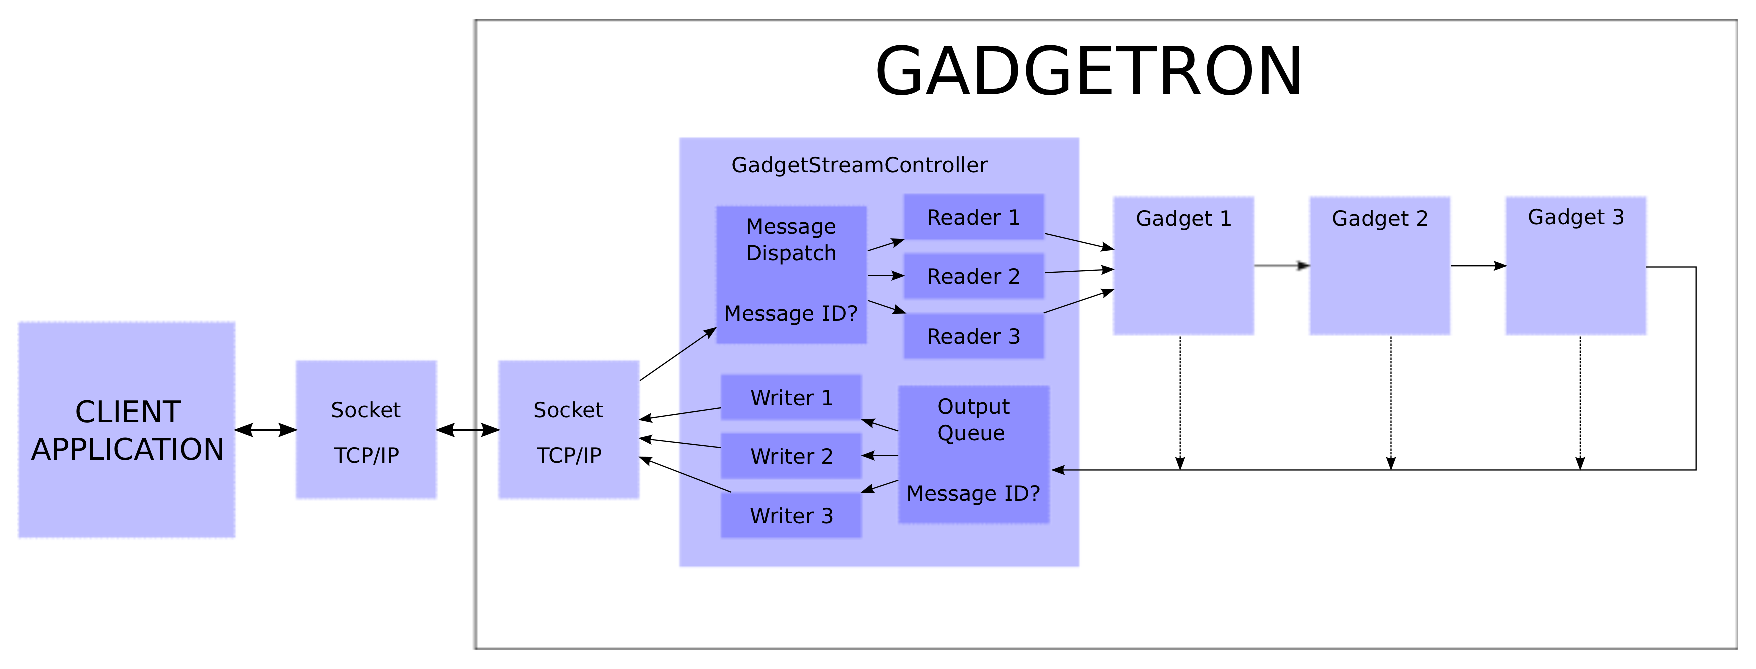
\includegraphics[width=6in]{figures/architecture.eps} 
   \caption{Overview of Gadgetron architecture.}
   \label{fig:architecture}
\end{figure}

\subsection{Gadgetron XML Configuration}
\label{section:gadgetxmlconfiguration}
The Gadgetron can be configured dynamically using an XML script. Specifically, the Gadgetron employs dynamic runtime linking to assemble a system of Readers, Writers and Gadgets. These components can be assembled from multiple different shared libraries (DLLs on Windows or Shared Objects on Linux/Unix systems). An example XML configuration file can be seen below:

{\scriptsize 
\begin{verbatim}
<?xml version="1.0" ?>  

<readers>
<reader slot="1001" dll="gadgetroncore" class="MRIAcquisitionReader" />
</readers>

<writers>
<writer slot="1004" dll="gadgetroncore" class="MRIImageWriter" />
</writers>

<stream>
<gadget name="ImageFinish" dll="gadgetroncore" class="ImageFinishGadget" />
<gadget name="CropCombine" dll="gadgetroncore" class="CropAndCombineGadget" />
<gadget name="FFT" dll="gadgetroncore" class="FFTGadget" />
<gadget name="Acc" dll="gadgetroncore" class="AccumulatorGadget" /> 
<gadget name="NoiseAdjust" dll="gadgetroncore" class="NoiseAdjustGadget" />
</stream>
\end{verbatim} 
}

There are 3 main sections to the configuration matching the 3 types of components that need to be configured: Readers, Writers and the Gadgets. In the Readers section there is one reader registered, it is assigned to message ID (or slot) number 1001. The user can in principle pick these IDs freely, but there are certain reserved IDs for configuration information, etc. and it is recommended not to use IDs below 1000. The XML configuration informs the Gadgetron to load a class called \texttt{MRIAcquisitionReader} from the shared library called \texttt{gadgetroncore}, i.e. \texttt{gadgetroncore.dll} on Windows, \texttt{libgadgetroncore.so} on Linux, or \texttt{libgadgetron.dylib} on Mac OS X. The next section configures the Writers, in this case there is only one Writer associated with the Gadgetron and it is associated with message ID or slot number 1004. The Reader and Writer slot numbers are independent, but similarly to the Readers it is recommended not to use IDs below 1000.

The \texttt{stream} section of configuration defines which Gadgets will get inserted in the stream. The Gadget stream configuration is read in order and pushed onto the stream (;oke a stack) such that the first Gadget in the stream will effectively be the last one in the configuration list. This may be somewhat counterintuitive but is is a principle which is inherited from the ACE framework that the Gadgetron is built on. Each Gadget is given a name which can be used later to locate a specific Gadget. Similarly to the Readers and Writers the user must specify which shared library the Gadget can be found in and the name of the class to be loaded from that shared library. 

The XML configuration provides a flexible way of assembling and modifying Gadget chains without having to recompile the Gadgetron. In fact, this XML configuration can be supplied from the outside by the client application, thus allowing clients to configure the Gadgetron dynamically based on the type of data it would like to send. See section \ref{section:builtinmessages} for details on how to send the Gadgetron XML configuration from the client. 

\subsection{Socket Communication Protocol}
\label{section:socketcommunicationprotocol}
The Gadgetron uses a very simple communication protocol with virtually no overhead. The Gadgetron continuously reads messages of the socket. Each reads starts with reading a \texttt{GadgetMessageIdentifier}:
{\scriptsize 
\begin{verbatim}
struct GadgetMessageIdentifier
{
  ACE_UINT16 id;
};
\end{verbatim}}
The  GadgetMessageIdentifier consists of just one 16-bit unsigned integer which is used to tell the Gadgetron which Reader to call up to read this message. As described in section \ref{section:gadgetxmlconfiguration} a Reader must be registered for each type of message that is sent to the Gadgetron. If an unknown message ID is received, the GadgetStreamController will fail and close the connection to the client. 

There are a number of built in message IDs that are used to enable clients to send configuration details and parameters to the Gadgets. Specifically, the following messages are defined:
{\scriptsize 
\begin{verbatim}
enum GadgetronMessageID {
  GADGET_MESSAGE_INT_ID_MIN       =   0,
  GADGET_MESSAGE_CONFIG_FILE      =   1,
  GADGET_MESSAGE_CONFIG_SCRIPT    =   2,
  GADGET_MESSAGE_PARAMETER_SCRIPT =   3,
  GADGET_MESSAGE_INT_ID_MAX       = 999
};
\end{verbatim}}

The message ID \texttt{GADGET\_MESSAGE\_CONFIG\_FILE} is used to indicate that the following message is the filename of an XML configuration file (see section \ref{section:gadgetxmlconfiguration}) on the Gadgetron host. The Gadgetron has a built in Reader associated with this ID and it finds and reads the XML configuration file specified in the data structure: 
{\scriptsize 
\begin{verbatim}
struct GadgetMessageConfigurationFile
{
  char configuration_file[1024];
};
\end{verbatim}}
Alternatively the client can use the \texttt{GADGET\_MESSAGE\_CONFIG\_SCRIPT} to specify that the XML configuration will be transmitted from the client. A built-in reader is also associated with this ID and it reads a struct which specifies the length of the XML configuration and then an XML stream as specified:
{\scriptsize 
\begin{verbatim}
struct GadgetMessageScript
{
  ACE_UINT32 script_length;
};
\end{verbatim}}

The last predefined ID is  \texttt{GADGET\_MESSAGE\_PARAMETER\_SCRIPT } for which a built-in Reader is also registered. It will also read a  \texttt{GadgetMessageScript} struct to determine the length of the parameter script to follow and then read a stream of characters of that length. The Gadgetron does not assume anything about the format of the parameter script, it is passed on to every Gadget without modification as described in section \ref{section:gadgets}. It is up to each individual Gadget how this script is to be interpreted. The convention has been to pass an XML script with parameters and the Gadgetron includes utility functions for reading XML configuration documents, but the user may chose a different format for the configuration if needed. However, it is passed to all Gadgets in the chain and it is the responsibility of the user to ensure that the parameters can be understood by all Gadgets in the chain. 

\subsection{Gadgets}
\label{section:gadgets}
Gadgets are active objects (see figure \ref{fig:gadget}). They have their own execution thread, in fact they may have multiple execution threads\footnote{For users familiar with ACE, Gadgets are based on the \emph{ACE\_Task} class.} . Each Gadget has a message queue where messages passed from upstream Gadgets (or Readers) are placed. Each message is comprised of one or more message blocks that are linked together. The message blocks are based on the ACE\_Message\_Block class which is basically a reference counted raw buffer with a few utility functions for chaining messages together and for determining the size, etc. of the message. In principle it is possible to implement Gadgets that act on these basic message blocks. All that is needed is to implement a class which inherits from Gadget (as defined in \texttt{Gadget.h}):

{\scriptsize 
\begin{verbatim}
class MyGadget : public Gadget
{
protected:
  virtual int process(ACE_Message_Block *m)
  {
    
    //Do something with the message block
    
    m->release();
    return GADGET_OK;
  }
};
\end{verbatim}}

\noindent
The problem with this approach is that there is no reliable way to check inside the Gadget if the right data type is being received and since the message blocks are really just raw blocks of memory, there is a potential for crashes that can be hard to track down. To overcome this problem the message blocks are typically of the type \texttt{GadgetContainerMessage<T>} which is a templated class based on \texttt{ACE\_Message\_Block} which is designed to a) package an object of any type (as long as it has a default constructor which take no arguments) and pack it into an \texttt{ACE\_Message\_Block} and b) provide functionality for checking if a given message block on the message queue is a \texttt{GadgetContainerMessage} containing a given type. This datatype is described in more detail in section \ref{section:gadgetcontainermessage}, but the most important feature is that there is a templated function:
{\scriptsize 
\begin{verbatim}
template <class T> GadgetContainerMessage<T>* AsContainerMessage(ACE_Message_Block* mb)
\end{verbatim}}
\noindent
which will allow the user to take a given message block in a Gadget and attempt to convert it to a \texttt{GadgetContainerMessage} of a given type and this function will return a pointer to the \texttt{GadgetContainerMessage} if successful and zero otherwise. After conversion it is possible to access the packed object (as given by type \texttt{T}) using the \texttt{GetObjectPtr()} function on the \texttt{GadgetContainerMessage}. This is illustrated in the following code:
{\scriptsize 
\begin{verbatim}
class MyGadget : public Gadget
{
protected:
  virtual int process(ACE_Message_Block *m)
  {
    
    GadgetContainerMessage<MyType>* cm = AsContainerMessage<MyType>(m);
    
    if (!cm) {
         GADGET_DEBUG1("Failed to convert message block\n");
         m->release();
         return GADGET_FAIL;
    } 
    
    //Do something with the data
    cm->GetObjectPtr()-> .....
    
    m->release();
    return GADGET_OK;
  }
};
\end{verbatim}}

\begin{figure}[htbp] %  figure placement: here, top, bottom, or page
   \centering
   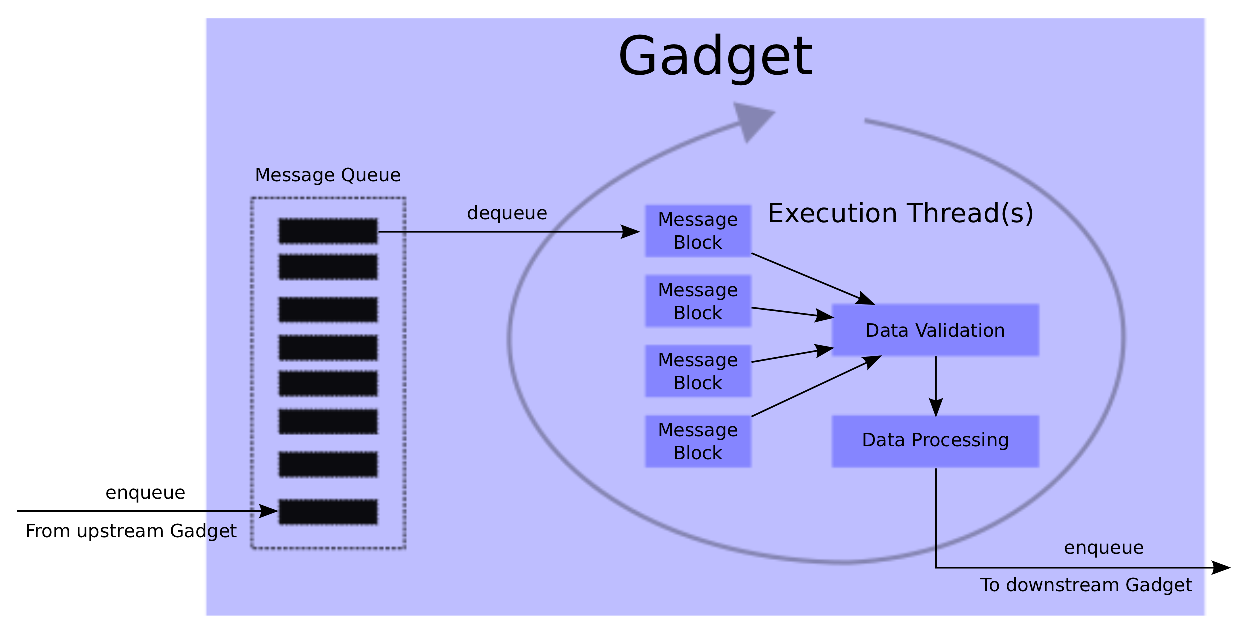
\includegraphics[width=6in]{figures/gadget.eps} 
   \caption{Basic Gadget Architecture}
   \label{fig:gadget}
\end{figure}

\subsubsection{Predefined Multi Parameter Gadgets}
To make it even easier create new Gadgets and ensure that appropriate data is passed between Gadgets some predefined Gadgets have been created that a) automatically process the raw message block and check data types and b) pass the data onto a process function which takes the appropriate data types. For instance the Gadgetron predefines \texttt{Gadget1<T>} like this:

{\scriptsize 
\begin{verbatim}
template <class P1> class Gadget1 : public Gadget
{
  
protected:

  //Omitted functions....

  virtual int process(GadgetContainerMessage<P1>* m) = 0;

};
\end{verbatim}}

\noindent
In order to implement a Gadget which processes a data type called \texttt{MyType} all that is needed is the following code:
{\scriptsize 
\begin{verbatim}
class MyProcessingGadget : public Gadget1<MyType>
{  
protected:

virtual int process(GadgetContainerMessage<MyType>* m)
  {
  
       //Do something with data
       
      m->release();
      return GADGET_OK;
  }
};
\end{verbatim}}

\noindent
It is guaranteed that by the time the \texttt{process(...)} is called the data has been checked and is ready for processing. 

\subsubsection{Gadget Configuration}
A given application or client may need to configure the Gadgets in the chain to match a given data acquisitions (e.g. number of data points, image size, etc.). There are two mechanisms for passing parameters to the Gadgets: a) Through the XML configuration file or b) with a parameter script (of arbitrary format) as briefly mentioned in section \ref{section:socketcommunicationprotocol}.

Gadgets can have parameters set in the XML configuration with syntax like:
{\scriptsize 
\begin{verbatim}
<gadget name="Grappa" dll="gadgetrongrappa" class="GrappaGadget"> 
<property name="uncombined_channels" value="15" />
</gadget>
\end{verbatim}}
\noindent
In this case the "Grappa" Gadget will have a parameter called \texttt{uncombined\_channels} set to the value 15. The Gadget properties are available from within the Gadget using the following member functions:
{\scriptsize 
\begin{verbatim}
//Setting parameters
int set_parameter(const char* name, const char* val);

//Accessing parameters
int get_bool_value(const char* name);
int get_int_value(const char* name);
double get_double_value(const char* name);
boost::shared_ptr<std::string> get_string_value(const char* name);
\end{verbatim}}

The second mechanism for passing configuration information is by sending a script with the message ID \texttt{GADGET\_MESSAGE\_PARAMETER\_SCRIPT }. The predefined parser associated with this ID will ensure that the message block data is marked in such a way that it will not pass to the \texttt{process(...)} function of the Gadget but to a \texttt{process\_config(....)} function, which has a default implementation:
{\scriptsize 
\begin{verbatim}
  virtual int process_config(ACE_Message_Block * m) {
    return 0;
  }
\end{verbatim}}
\noindent
It is up to the user to override this default implementation if the Gadget should have a particular behavior when receiving configuration information. As mentioned previously there are no predefined requirements for the formatting of this parameter script, it could even be binary configuration data. However, it is important to remember that this script is passed to all Gadgets in the chain and it is good practice to use a consistent format such as XML that will allow each individual Gadget to use the parameters that it may need and ignore the others. 

\subsection{Readers and Writers}
The Readers and Writers control the input and output from the Gadgetron. It is easy to implement support for new data types by implementing the following interfaces:
{\scriptsize 
\begin{verbatim}
class GadgetMessageReader
{
 public:
  virtual ACE_Message_Block* read(ACE_SOCK_Stream* stream) = 0;
};

class GadgetMessageWriter
{
 public:
  virtual int write(ACE_SOCK_Stream* stream, ACE_Message_Block* mb) = 0;
};
\end{verbatim}}
\noindent
As is seen the Reader will be handed a socket to read from and its job is to deserialize the message on the socket and pack it nicely into a chain of \texttt{ACE\_Message\_Block}. A pointer to the first message block is returned to the Gadgetron and passed down the chain of Gadgets. Writers perform the opposite operation they receive a message in the form of a chain of message blocks and it is the job of the Writer to serialize this chain of message blocks and write the data onto the provided socket.

\section{Toolboxes}


\section{Examples}

\renewcommand{\refname}{\section{References}}
\bibliography{references/references}{}
\bibliographystyle{plain}

\section{Appendix - The Gory Details}
\subsection{Organization of Files}
\subsection{XML Configuration Syntax}
\subsection{GadgetContainerMessage}
\label{section:gadgetcontainermessage}

\end{document}  